%%%%%%%%%%%%%%%%%%%%%%%%%%%%%%%%%%%%%%%%%%%%%%%%%%%%%%%%%%%%%%%%%%%%%%%
%% template for II2202 report
%% original 2015.11.24
%% revised  2016.08.23
%%%%%%%%%%%%%%%%%%%%%%%%%%%%%%%%%%%%%%%%%%%%%%%%%%%%%%%%%%%%%%%%%%%%%%%
%

\title{Comparison of software and hardware video codecs from perspective of power consumption}
\author{
        \textsc{Jaroslav Svoboda}
            \qquad
        \textsc{Michel Muffei}
        \mbox{}\\
        \normalsize
            \texttt{svoboda}
        \textbar{}
            \texttt{mmuffei}
        \normalsize
            \texttt{@kth.se}
}
\date{\today}

\documentclass[12pt,twoside]{article}

\usepackage[paper=a4paper,dvips,top=1.5cm,left=1.5cm,right=1.5cm,
    foot=1cm,bottom=1.5cm]{geometry}


%\usepackage[T1]{fontenc}
%%\usepackage{pslatex}
\renewcommand{\rmdefault}{ptm} 
\usepackage[utf8]{inputenc}
\usepackage{mathptmx}
\usepackage[scaled=.90]{helvet}
\usepackage{courier}
\usepackage[swedish,UKenglish]{babel}
\usepackage[gen]{eurosym}
\usepackage[UKenglish]{isodate}
\usepackage{selinput}
\usepackage{tabu}
\usepackage{multirow}
\usepackage{booktabs}
\usepackage[backend=biber]{biblatex}
\addbibresource{II2202-report.bib}
\usepackage{hyperref}
\usepackage{bookmark}
\usepackage[binary-units=true,per-mode=symbol]{siunitx}
\usepackage[acronym]{glossaries}
\usepackage{listings}
\makeglossaries

\usepackage{fancyhdr}
\pagestyle{fancy}

%%----------------------------------------------------------------------------
%%   pcap2tex stuff
%%----------------------------------------------------------------------------
 \usepackage[dvipsnames*,svgnames]{xcolor} %% For extended colors
 \usepackage{tikz}
 \usetikzlibrary{arrows,decorations.pathmorphing,backgrounds,fit,positioning,calc,shapes}

%% \usepackage{pgfmath}	% --math engine
%%----------------------------------------------------------------------------
%% \usepackage[latin1]{inputenc}
 % inputenc allows the user to input accented characters directly from the keyboard

%% \usepackage{rotating}		 %% For text rotating
\usepackage{array}			 %% For table wrapping
\usepackage{graphicx}	                 %% Support for images
\usepackage{float}			 %% Suppor for more flexible floating box positioning
\usepackage{color}                       %% Support for colour 
\usepackage{mdwlist}

\usepackage{dcolumn}	                 %% Support for decimal point alignment in tables
\usepackage{url}	                 %% Support for breaking URLs
\usepackage[perpage,para,symbol]{footmisc} %% use symbols to ``number'' footnotes and reset which symbol is used first on each page

%% \usepackage{pygmentize}           %% required to use minted -- see python-pygments - Pygments is a Syntax Highlighting Package written in Python
%% \usepackage{minted}		     %% For source code highlighting

%% \usepackage{hyperref}		
\usepackage[all]{hypcap}	 %% Prevents an issue related to hyperref and caption linking
%% setup hyperref to use the darkblue color on links
%% \hypersetup{colorlinks,breaklinks,
%%             linkcolor=darkblue,urlcolor=darkblue,
%%             anchorcolor=darkblue,citecolor=darkblue}

%% Some definitions of used colors
\definecolor{darkblue}{rgb}{0.0,0.0,0.3} %% define a color called darkblue
\definecolor{darkred}{rgb}{0.4,0.0,0.0}
\definecolor{red}{rgb}{0.7,0.0,0.0}
\definecolor{lightgrey}{rgb}{0.8,0.8,0.8} 
\definecolor{grey}{rgb}{0.6,0.6,0.6}
\definecolor{darkgrey}{rgb}{0.4,0.4,0.4}
%% Reduce hyphenation as much as possible
\hyphenpenalty=15000 
\tolerance=1000

%% useful redefinitions to use with tables
\newcommand{\rr}{\raggedright} %% raggedright command redefinition
\newcommand{\rl}{\raggedleft} %% raggedleft command redefinition
\newcommand{\tn}{\tabularnewline} %% tabularnewline command redefinition

%% definition of new command for bytefield package
\newcommand{\colorbitbox}[3]{%
	\rlap{\bitbox{#2}{\color{#1}\rule{\width}{\height}}}%
	\bitbox{#2}{#3}}

%% command to ease switching to red color text
\newcommand{\red}{\color{red}}
%%redefinition of paragraph command to insert a breakline after it
\makeatletter
\renewcommand\paragraph{\@startsection{paragraph}{4}{\z@}%
  {-3.25ex\@plus -1ex \@minus -.2ex}%
  {1.5ex \@plus .2ex}%
  {\normalfont\normalsize\bfseries}}
\makeatother

%%redefinition of subparagraph command to insert a breakline after it
\makeatletter
\renewcommand\subparagraph{\@startsection{subparagraph}{5}{\z@}%
  {-3.25ex\@plus -1ex \@minus -.2ex}%
  {1.5ex \@plus .2ex}%
  {\normalfont\normalsize\bfseries}}
\makeatother

\setcounter{tocdepth}{3}	%% 3 depth levels in TOC
\setcounter{secnumdepth}{5}
%%%%%%%%%%%%%%%%%%%%%%%%%%%%%%%%%%%%%%%%%%%%%%%%%%%%%%%%%%%%%%%%%%%%
%% End of preamble
%%%%%%%%%%%%%%%%%%%%%%%%%%%%%%%%%%%%%%%%%%%%%%%%%%%%%%%%%%%%%%%%%%%%

\renewcommand{\headrulewidth}{0pt}
\lhead{II2202, Fall 2016, Period 1-2}
%% or \lhead{II2202, Fall 2016, Period 1}
\chead{Draft project report}
\rhead{\date{\today}}

\makeatletter
\let\ps@plain\ps@fancy 
\makeatother

\setlength{\headheight}{15pt}
\begin{document}

\maketitle


\begin{abstract}
\label{sec:abstract}

Your abstract here.

\end{abstract}
%%\clearpage


\tableofcontents
\newacronym{msssim}{MS-SSIM}{Multi-Scale Structural Similarity}
\newacronym{psnrhvsm}{PSNR-HVS-M}{Peak Signal-to-Noise Ratio taking into account Contrast Sensitivity Function (CSF) and between-coefficient contrast masking of DCT basis functions}
\newacronym{vmaf}{VMAF}{Video Multi-Method Assessment Fusion}
\newacronym{vqmt}{VQMT}{Video Quality Measurement Tool}
\newacronym{nvidiasmi}{NVIDIA SMI}{NVIDIA System Management Interface}
\printglossary[type=\acronymtype]



\clearpage
\section{Introduction}
\label{sect:introduction}
Video encoding and decoding are processes with many variables which can influence the output of whole process of video transfer. Visual quality of video is determined by chosen coding standard, its implementation and encoding settings. All these three key elements have direct impact on energy resources we need for completing encode. Video coding standard defines complexity of algorithm and usually the more effective compression the more complex algorithm - the more power demanding. There are many types of implementations but usually the more hardwired algorithms it uses the less power demanding it is. At last, used encoding settings determine time needed for compression. That also means power necessary for encode. From this point of view, power consumption one, it is interesting to create comparison of different video codecs to see how much quality of video costs in used energy.


\subsection{Theoretical framework/literature study}
\label{sect:framework}


We had to compile FFmpeg with support of NVENC and QSV.\cite{intelffmpeg,nvidiaffmpeg}

\subsubsection{\acrfull{psnrhvsm}}
In dB. More is better.
\subsubsection{\acrfull{msssim}}
From 0 to 1. More is better.
\subsubsection{\acrfull{vmaf}}
Newly developed metric by Netflix. Based on machine learning. From 0 to 100. More is better.

\subsection{Research questions, hypotheses}
\label{sect:questions}
Hardware accelerated codecs are faster but with lower quality and lower power consumption.


\section{Method}
\label{sec:method}
We choose three test sequences, each \num{500} frames long.  More in table \ref{tab:sequences}
\begin{table}[h]
	\centering
	\caption{Parameters of test sequences}
	\label{tab:sequences}
	\begin{tabu}{lrrr}
		\toprule[2pt]
		Sequence     & crowd\_run\_2160p50.y4m & old\_town\_cross\_2160p50.y4m & sintel.y4m \\
		\midrule
		Resolution   & $3840\times2160$               & $3840\times2160$  & $4096\times1744$  \\
		framerate    & $50$p                     & $50$p                 & $24$p        \\
		\# of frames & $500$                     & $500$                 & $500$        \\
		subsampling & $4:2:0$	&	$4:2:0$	&	$4:2:0$ \\
		size in bytes &\num{6220803036}&\num{6220803036}&    \num{5357571060}      \\
		\bottomrule[2pt]  
	\end{tabu}
\end{table}

Whole process was done for all codecs as follows:
\begin{enumerate} 
	\item Power measuring tools are enabled
	\item Encoding proceeds
	\item Power measuring tools are disabled
	\item Encoded video is trans-coded to YUV420P
	\item Quality is measured
\end{enumerate}
This is done for all three chosen sequences, all chosen codecs and all presets available in bit-rates from \textsc{\SI{500}{\kilo\bit\per\second}} to \SI{5000}{\kilo\bit\per\second} with \SI{500}{\kilo\bit} steps and then up to \SI{15000}{\kilo\bit\per\second} with \SI{1000}{\kilo\bit} steps. Total number of encodes is (1080 so far). For quality evaluation we chose 3 methods: \acrshort{psnrhvsm} and \acrshort{msssim}, both measured by \acrshort{vqmt}, and then \acrshort{vmaf}. Power consumption was measured by Intel Power Gadget which provides cumulative energy consumption in \SI{}{\milli\watt\hour}. Power consumption of GPU was measured by \acrfull{nvidiasmi}. Because this tool does not provide cumulative values, measurement was done \SI{1}{\second} intervals and then summed and converted to \SI{}{\milli\watt\hour}.

Information about used software provides table \ref{tab:sw}. Information about used hardware provides table \ref{tab:hw}.
\begin{table}[h]
	\centering
	\caption{Used software}
	\label{tab:sw}
	\begin{tabu}{ll}
		\toprule[2pt]
		Name                               & Version  \\
		\midrule
		Ubuntu GNOME                       & 16.04.1 LTS   \\
		Mesa                               &   13.0     \\
		Nvidia driver                               &    375    \\
		FFmpeg                             &           \\
		x264                               &          \\
		x265                               &          \\
		OpenH264                           &          \\
		libtheora                          &         \\
		libvpx                             &         \\
		\acrshort{nvidiasmi} &          \\
		Intel Power Gadget                 &       \\
		\acrshort{vmaf} Development Kit               &          \\
		\acrshort{vqmt}                               &        \\
		\bottomrule[2pt]
	\end{tabu}
\end{table}

\begin{table}[h]
	\centering
	\caption{Used hardware}
	\label{tab:hw}
	\begin{tabu}{ll}
		\toprule[2pt]
		Part                               & Specification \\
		\midrule
		CPU                      & Intel Core i5-4570@\SI{3.2}{\giga\hertz}   \\
		RAM                             &   DDR3 \SI{32}{\giga\byte}     \\
		GPU                               & Nvidia 960 GTX \SI{4}{\giga\byte}         \\
		SSD                               & Samsung EVO 850 \SI{250}{\giga\byte}      \\
		\bottomrule[2pt]
	\end{tabu}
\end{table}
\section{Results and Analysis}
\label{sec:results}
\subsection{h264\_nvenc}

\begin{figure}[!h]
	\vspace{-10pt}
	\centering
	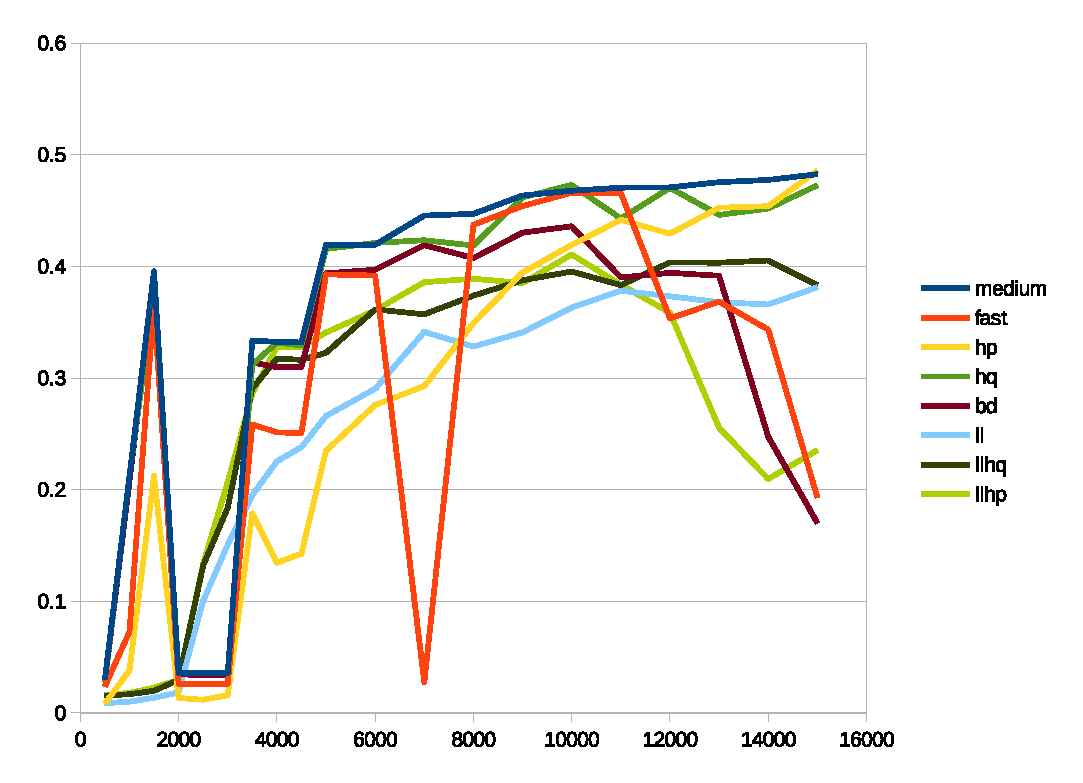
\includegraphics[width=0.9\textwidth]{img/h264_nvencoldtTownCrossPCR.eps}
	\caption{h264\_nvenc PCR for old\_town\_cross}
	\label{fig:h264_nvencoldtTownCrossPCR}
\end{figure}
\begin{figure}[!h]
	\vspace{-10pt}
	\centering
	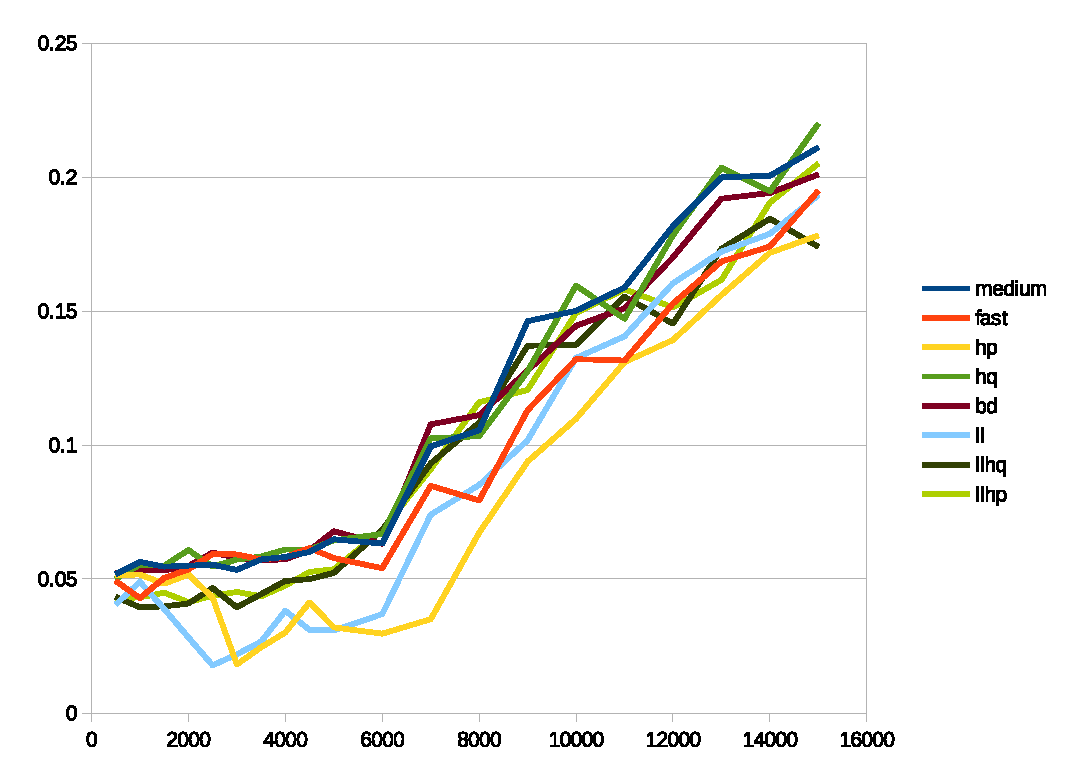
\includegraphics[width=0.9\textwidth]{img/h264_nvencCrowdRunPCR.eps}
	\caption{h264\_nvenc PCR for crowd\_run}
	\label{fig:h264_nvencCrowdRunPCR}
\end{figure}
\begin{figure}[!h]
	\vspace{-10pt}
	\centering
	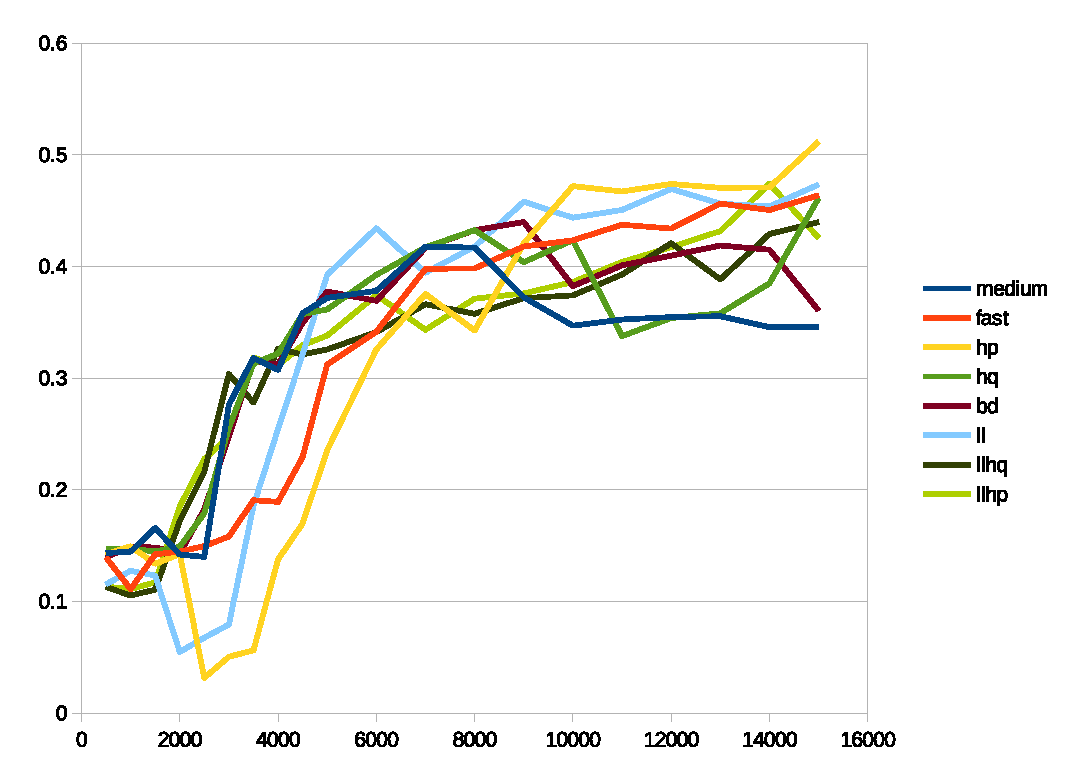
\includegraphics[width=0.9\textwidth]{img/h264_nvencSintelPCR.eps}
	\caption{h264\_nvenc PCR for sintel}
	\label{fig:h264_nvencSintelPCR}
\end{figure}
\subsection{x264}
\begin{figure}[!h]
	\vspace{-10pt}
	\centering
	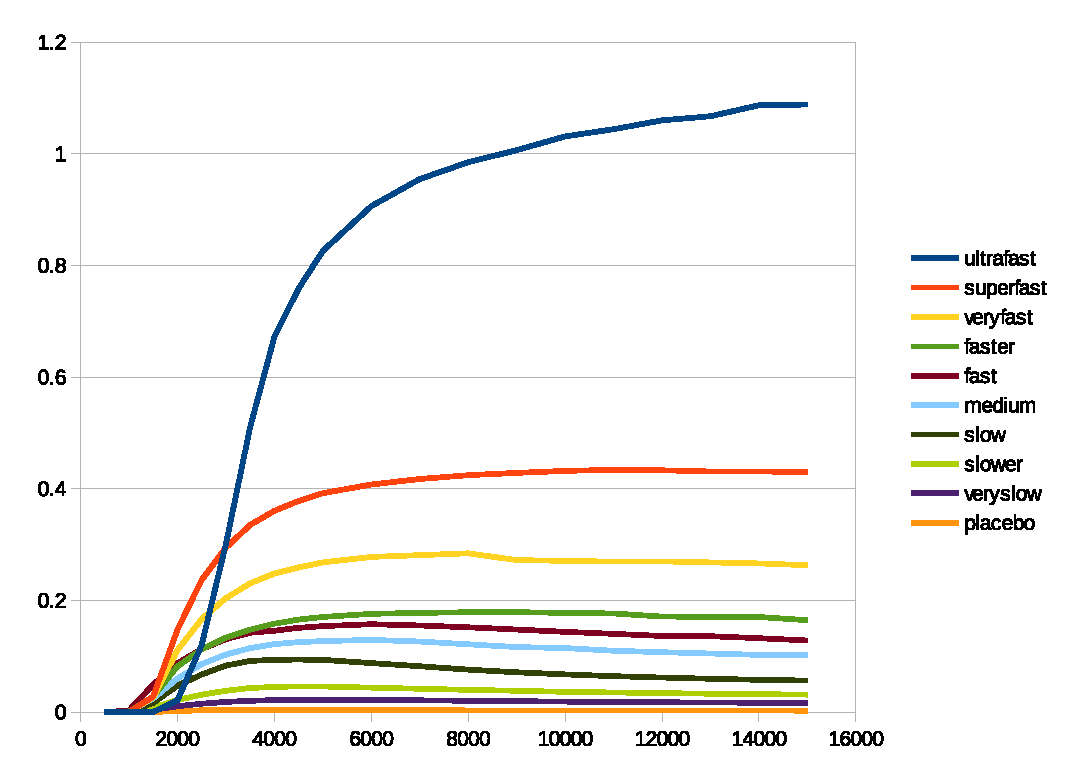
\includegraphics[width=0.9\textwidth]{img/x264oldtTownCrossPCR.eps}
	\caption{x264 PCR for old\_town\_cross}
	\label{fig:x264oldtTownCrossPCR}
\end{figure}
\newpage
\section{Discussion}
\label{sec:discussion}
xxxxx xxxx xxxx 
\newpage
\printbibliography
\appendix
\section{Annex}
%Compile script
%\lstinputlisting[frame=single,breaklines=true]{compile.sh}
Encoding script
\lstinputlisting[frame=single,breaklines=true]{encoding.sh}

\end{document}
